\documentclass[10pt]{beamer}

\usepackage{mathtools}
\usepackage{bm}
\usetheme{CambridgeUS}
\usecolortheme{dolphin}

\usepackage{graphicx}
\graphicspath{ {./images/} }

\usepackage{longtable}
\usepackage{booktabs}
\usepackage{multirow}
\usepackage{subfig}
\usepackage{caption}
\usepackage{float}

\usepackage{comment}

\usepackage{natbib}
\bibliographystyle{unsrtnat}
\setcitestyle{authoryear, open={(}, close={)}}

% set colors
\definecolor{myNewColorA}{RGB}{115, 0, 10} % garnet
\setbeamercolor*{palette primary}{bg=myNewColorA, fg=white}
\setbeamercolor*{palette secondary}{bg=myNewColorA, fg=white}
\setbeamercolor*{palette tertiary}{bg=myNewColorA, fg=white}
\setbeamercolor*{titlelike}{fg=myNewColorA}
\setbeamercolor*{title}{bg=myNewColorA, fg = white}
\setbeamercolor*{item}{fg=myNewColorA}
\setbeamercolor*{caption name}{fg=myNewColorA}
\usefonttheme{professionalfonts}

\titlegraphic{
\includegraphics[height=1.5cm]{images/usc_logo.png}}

\setbeamerfont{title}{size=\large}
\setbeamerfont{subtitle}{size=\small}
\setbeamerfont{author}{size=\small}
\setbeamerfont{date}{size=\small}
\setbeamerfont{institute}{size=\small}

\title[Modeling Stolen Base Outcomes]{Modeling the Probability of a Successful Stolen Base Attempt in Major League Baseball}
\author[Cade Stanley]{Cade Stanley \\{\scriptsize Director of Thesis: Dr. Joshua Tebbs} \\{\scriptsize Second Reader: Dr. Ting Fung Ma}}

\institute[University of South Carolina]{University of South Carolina Honors College}
\date[April 13, 2023]{April 13, 2023}

%------------------------------------------------------------
%This block of commands puts the table of contents at the 
%beginning of each section and highlights the current section:
%\AtBeginSection[]
%{
%  \begin{frame}
%    \frametitle{Contents}
%    \tableofcontents[currentsection]
%  \end{frame}
%}

\AtBeginSection[]{
  \begin{frame}
  \vfill
  \centering
  \begin{beamercolorbox}[sep=8pt,center,shadow=true,rounded=true]{title}
    \usebeamerfont{title}\insertsectionhead\par%
  \end{beamercolorbox}
  \vfill
  \end{frame}
}
%------------------------------------------------------------

\begin{document}
\frame{\titlepage}

%\begin{frame}
%\frametitle{Contents}
%\tableofcontents
%\end{frame}
%------------------------------------------------------------
\section{Introduction}
\begin{frame}{Background}
\begin{itemize}
    \item In sports, teams constantly search for a competitive edge
    \begin{itemize}
        \item In the front office: evaluating talent, spending money wisely

        \item On the field: selecting optimal lineups and strategies, making sound in-game decisions
    \end{itemize}
    \vspace{3mm}
    \item An important decision made several times a game in the MLB: whether to attempt to steal second base
    \begin{itemize}
        \item Success: the runner reaches ``scoring position,'' where any hit will likely score the runner

        \item Failure: the runner is removed from the basepaths, and an out is recorded
    \end{itemize}
\end{itemize}
\end{frame}

\begin{frame}{Existing Research}
\begin{itemize}
    \item Existing research: identifying the minimum success rate needed for stolen base attempts to be worthwhile
    \begin{itemize}
        \item Failed attempts are more harmful than successful attempts are helpful
    
        \item In general: success rate of 75\% is needed to add positive value \citep{Stolen-Base-Percentage}

        \item \cite{keyes}: identifies ``breakeven'' success rate for specific situations (according to the number of outs and the runners on base)
    \end{itemize}
    \vspace{3mm}
    \item Less focus on estimating the probability of success of a particular stolen base attempt
    \begin{itemize}
        \item With an estimate of the likelihood of success, previous research can be used to make a decision rule for attempting to steal
    \end{itemize}
\end{itemize}
\end{frame}

\begin{frame}{Approach}
\begin{itemize}
    \item Binary classification models -- logistic regression and random forests
    \vspace{3mm}
    \item Use data about the game situation and the players involved in the stolen base attempt to predict the outcome
    \begin{itemize}
        \item Baserunner speed, catcher arm strength

        \item Pitcher and batter handedness

        \item Number of outs, number of balls and strikes

        \item Number of pickoff throws, number of pitchouts

        \item Presence of a runner on third base

        \item Type and speed of the pitch thrown
    \end{itemize}
    %\vspace{1mm}
    %\item Use estimated probability of success to make decisions
    %\begin{itemize}
    %    \item Following \cite{keyes} and \cite{stoll}: 
        %\begin{itemize}
        %    \item calculate the estimated change in expected runs from a stolen base attempt
            
        %    \item attempt to steal if this change is positive
        %\end{itemize}
    %\end{itemize}
\end{itemize}
\end{frame}



\section{Methodology}
\begin{frame}{Data Collection}
\begin{itemize}
    \item Retrosheet's play-by-play game files
    \begin{itemize}
        \item Lineups, at-bats, and plays from every game of the 2018 MLB season

        %\item Used to document the game situation and result of every stolen base attempt
    \end{itemize}
    \vspace{3mm}
    \item Paul Schale's pitch data sets on Kaggle
    \begin{itemize}
        \item Type, speed, and location data for every pitch from the 2018 MLB season

        %\item Used to document pitch data (in particular, pitch speed) for pitches thrown during stolen base attempts
    \end{itemize}
    \vspace{3mm}
    \item Baseball Savant's Statcast data sets
    \begin{itemize}
        \item Player attributes, including baserunner speed and catcher arm strength

        \item Measures of players' historical success with stolen base attempts (2017 season)
    \end{itemize}
    \vspace{3mm}
    \item Baseball Reference's player data sets
    \begin{itemize}
        \item Success rates for catchers at defending against stolen bases in 2017 (not included in Statcast data)
    \end{itemize}
\end{itemize}
\end{frame}

\begin{frame}{Data Processing}
\begin{itemize}
    \item \textbf{Goal:} record the game situation at the time of every stolen base attempt during the 2018 season
    \vspace{3mm}
    \item \textbf{Problem:} Retrosheet event files are fairly simple -- they only encode the batter name, the sequence of pitches, and the outcome for each play
    \vspace{3mm}
    \item \textbf{Solution:} Use Python scripts to keep an updated account of the game situation after each play
    \begin{itemize}
        \item Record the kinds of pitches preceding each play

        \item Update the number of outs after each play
        
        \item Track the movement of runners around the basepaths

        \item Log any substitutions of pitchers, catchers, and baserunners
    \end{itemize}
\end{itemize}
\end{frame}

\begin{frame}{Data Processing -- Example 1}
\begin{figure}
    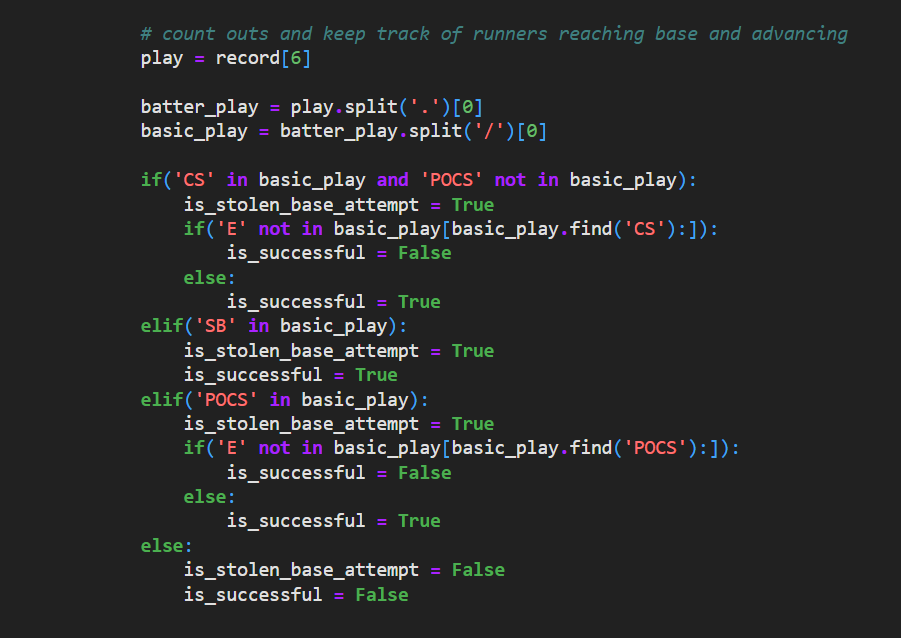
\includegraphics[height=2.5in]{images/code_example_1.png}
    \caption{Python code to identify stolen base attempts in the Retrosheet play-by-play data.}
    \label{code_example_1}
\end{figure}
\end{frame}

\begin{frame}{Data Processing -- Example 2}
\begin{figure}
    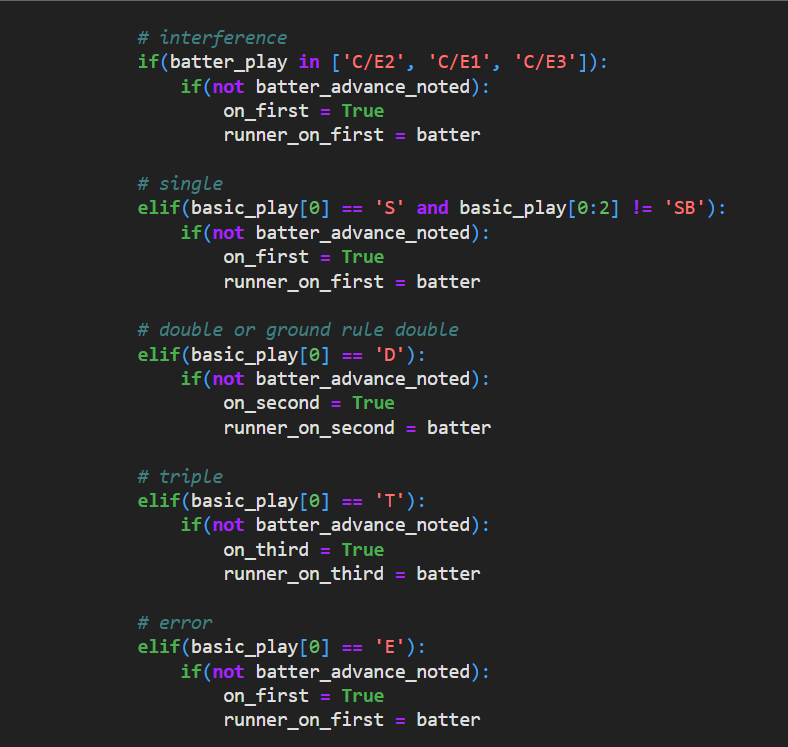
\includegraphics[height=2.5in]{images/code_example_2.png}
    \caption{Python code to log a play and record the batter's advance to the appropriate base.}
    \label{code_example_2}
\end{figure}
\end{frame}

\begin{frame}{Data Merging}
\begin{itemize}
    \item With the game situation of every stolen base attempt recorded, it remained to merge the rest of the data
    \vspace{3mm}
    \item Match pitch data (Kaggle) with the stolen base attempt on which it occurred
    \begin{itemize}
        \item merge on the game (home team, away team, date/time), the batter, the number of outs, and the number of pitches in the at-bat 
    \end{itemize}
    \vspace{3mm}
    \item Match player data (Statcast, Baseball Reference) with each stolen base attempt involving that player
    \begin{itemize}
        \item Merge on player names
        
        \item Some name discrepancies -- corrected these by hand
    \end{itemize}
\end{itemize}
\end{frame}

\begin{frame}{Data Analysis}
\begin{itemize}
    \item Using pitch data improves prediction, but has problems:
    \begin{itemize}
        \item Introduces missing observations -- about 200 (out of 2800) stolen base attempts did not occur on a pitch

        \item Cannot be used for making in-game decisions -- coaches and players cannot know what kind of pitch is coming
    \end{itemize}
    \vspace{3mm}
    \item Solution: perform the analysis with two data sets -- one with pitch data and one without
    \vspace{3mm}
    \item Train a logistic regression model and a random forest on each of the two data sets, for a total of four models
    \begin{itemize}
        \item Use cross-validation to evaluate prediction performance
    \end{itemize}
\end{itemize}
\end{frame}


\section{Results}
\begin{frame}{Model Performance}
    \begin{longtable}{c c c}
        \hline
        & Logistic Regression & Random Forest \\
        \hline
        AUC & \textbf{0.6915} & 0.6561 \\
        Prediction Accuracy & 0.7611 & \textbf{0.7613} \\
        Sensitivity & 0.9678 & \textbf{0.9684} \\
        Specificity & 0.1574 & 0.1564 \\
        \hline
        \caption{Performance of the models including the pitch data.}
        \label{results_tab1}
    \end{longtable}
    \begin{longtable}{c c c}
        \hline
        & Logistic Regression & Random Forest \\
        \hline
        AUC & 0.6759 & 0.6638 \\
        Prediction Accuracy & 0.7245 & 0.7361 \\
        Sensitivity & 0.9585 & 0.9400 \\
        Specificity & 0.1381 & \textbf{0.2253} \\
        \hline
        \caption{Performance of the models excluding the pitch data.}
        \label{results_tab2}
    \end{longtable}
\end{frame}

\begin{comment}
\begin{frame}{Variable Importance}
\begin{itemize}
    \item Logistic regression: most important variables are those included in the final model after stepwise variable selection and those with a very small p-value
    \begin{itemize}
        \item number of pitches in the at-bat
        \item speed of the pitch during the stolen base attempt
        \item baserunner's average sprint speed
        \item whether there is a runner on third
        \item whether the count is a hitter's count
    \end{itemize}

    \item Random forests: most important variables are measured using mean decrease in accuracy and mean decrease in Gini index
    \begin{itemize}
        \item number of pitches in the at-bat
        \item speed of the pitch
        \item baserunner's average sprint speed
        \item whether there is a runner on third
        \item stolen base success rates for pitchers, catchers, and baserunners in 2017
        \item pitcher's rate of fastballs and rate of successful pickoff attempts
        \item catcher's average pop time
    \end{itemize}
\end{itemize}
\end{frame}
\end{comment}


\section{Conclusion}
%\begin{frame}{Applications}
%\begin{itemize}
%    \item 
%\end{itemize}
%\end{frame}

\begin{frame}{Limitations}
\begin{itemize}
    \item For predictors measuring a player's historical success, we only used data from the 2017 season
    \begin{itemize}
        \item Using full career data would better represent a player's ability and would reduce the number of missing values
    \end{itemize}
\vspace{3mm}
    \item These models may not perform well in the aftermath of 2023 MLB rule changes
    \begin{itemize}
        \item Bigger bases, limits on pickoff throws may improve the viability of stolen base attempts in general

        \item Revisit these models, re-train them with data from 2023 and beyond
    \end{itemize}
\end{itemize}
\end{frame}

\begin{frame}{Future Work}
\begin{itemize}
    \item Improve model performance
    \begin{itemize}
        \item Explore additional predictors: pitcher's delivery time, runner's lead distance

        \item Try different methods: support vector machines, k-nearest neighbors, neural networks
    \end{itemize}
    \vspace{2mm}
    \item Identify an optimal cutoff value for classification
    \begin{itemize}
        \item Improve specificity to account for the cost of misclassifying an unsuccessful attempt as successful
    \end{itemize}
    \vspace{2mm}
    \item Evaluate the reliability of these models' probability estimates (not just their binary predictions)
    \begin{itemize}
        \item For example, stolen base attempts for which the models estimate a 70\% probability of success should be successful around 70\% of the time
    \end{itemize}
\end{itemize}
\end{frame}



\section{References}
\begin{frame}[allowframebreaks]{References}
    \nocite{*}
    \bibliography{references}
\end{frame}

\end{document}